\chapter[Random Walk Particle Tracking]{Random Walk Particle Tracking -- H- and Fluid Momentum- Process dependent}

\section{Theory}
\subsection{Governing Equation}\label{SS:GoverningEquation}
The classical advection-dispersion equation of a conservative solute in porous media can be written as \cite{jB79}

\begin{equation}\label{transport}
\frac{\partial C}{\partial t} = -\nabla(\textbf{V}C)+\nabla (\textbf{D} \nabla C)
\end{equation}

where $C$ is the concentration ($ML^{-3}$), $\textbf{V}$ is the pore velocity vector ($ML^{-1}$), and $\textbf{D}$ is the hydrodynamic dispersion tensor ($L^2T^{-1}$), t is time ($T^{2}$) and $ \nabla $is the differential operator.

The modified velocity \cite{wK86} and the dispersion tensor \cite{jB79} are expressed as

\begin{equation}\label{ModifiedVelocity}
V _i^* = V _i + \sum_{j=1}^{3}\frac{\partial D _{ij}}{\partial x _j}
\end{equation}

\begin{equation}\label{DispersionTensor}
D _{ij} = \alpha _T |\textbf{V}|\delta _{ij} + (\alpha _L - \alpha _T)\frac {V _i V _j}{|\textbf{V}|} + D^d _{ii}
\end{equation}
where $\delta _{ij}$ is the Kronecker symbol, $\alpha _L$ is the longitudinal dispersivity, $\alpha _T$ is the transverse dispersivity, $D^d _{ij}$ is the tensor of molecular diffusion coefficient, and $V _i$ is the component of the mean pore velocity in the $i$th direction.

The stochastic differential equation equivalent to (\ref{transport}) in three dimensional problems can be written as \cite{aT90,eL96,wK88}

\begin{equation}\label{StochasticDifferentialEquation}
\begin{array}{llllll}
x _{t+\Delta t} & =x _{t}+ \left(V _x(x _t,y _t,z _t,t) + \frac{\partial D _{xx}}{\partial x} + \frac{\partial D _{xy}}{\partial y} + \frac{\partial D _{xz}}{\partial z} \right ) \Delta t \\
&\quad + \sqrt{2D _{xx} \Delta t }Z _1 + \sqrt{2D _{xy} \Delta t }Z _2 + \sqrt{2D _{xz} \Delta t }Z _3 \\
y _{t+\Delta t} & =y _{t}+ \left(V _y(x _t,y _t,z _t,t) + \frac{\partial D _{yx}}{\partial x} + \frac{\partial D _{yy}}{\partial y} + \frac{\partial D _{yz}}{\partial z} \right ) \Delta t \\
&\quad + \sqrt{2D _{yx} \Delta t }Z _1 + \sqrt{2D _{yy} \Delta t }Z _2 + \sqrt{2D _{yz} \Delta t }Z _3 \\
z _{t+\Delta t} & =z _{t}+ \left(V _z(x _t,y _t,z _t,t) + \frac{\partial D _{zx}}{\partial x} + \frac{\partial D _{zy}}{\partial y} + \frac{\partial D _{zz}}{\partial z} \right ) \Delta t \\
&\quad + \sqrt{2D _{zx} \Delta t }Z _1 + \sqrt{2D _{zy} \Delta t }Z _2 + \sqrt{2D _{zz} \Delta t }Z _3 \\
\end{array}
\end{equation}

where $x$, $y$, and $z$ are the coordinates of the particle location, $\Delta t$ is the time step, and $Z _i$ is a random number whose mean is zero and variance is unit.

In equation (\ref{StochasticDifferentialEquation}), the spatial derivatives of the dispersion coefficients are introduced from the modified velocity \cite{wK86}. Together with equation (\ref{DispersionTensor}), the spatial derivatives of the dispersion coefficients can be expressed as a function of the derivatives of velocity. Note that to obtain the derivatives of velocity, velocity has to be continuous mathematically. For this end, we interpolate velocity at any location in an element from the known velocity at the element nodes. The velocity estimation and the interpolation method are provided in section \ref{SS:VELOCITY}.

Since the proposed RWPT method makes use of the FEM for velocity estimation, the derivative of velocity within each element is computed as in Figure \ref{DerivativeVelocity} and written as
\begin{equation}\label{DerivativeVelocityNotZero}
\begin{array}{ll}
\frac {\partial V _x}{\partial x} = & \frac {V(x_R) - V(x_L)}{l _x}; \quad
\frac {\partial V _y}{\partial y} = \frac {V(y _U) - V(y _D)}{l _y}; \quad
\frac {\partial V _z}{\partial z} = \frac {V(z _N) - V(z _S)}{l _z} \\
& \frac {\partial V _x}{\partial y} = \frac {\partial V _x}{\partial z} =
\frac {\partial V _y}{\partial z} = \frac {\partial V _y}{\partial x} =
\frac {\partial V _z}{\partial x} = \frac {\partial V _z}{\partial y}
\simeq 0
\end{array}
\end{equation}
where $x _L$ and $x _R$ are the intersectional points of the element edges with an extension of a  line parallel to the global $x$ axis at which velocities are $V(x _L)$ and $V(x _R)$, $y _D$ and $y _U$ are the intersectional points of the element edge from down to up with extension of the line parallel to the global $y$ axis at which velocities are $V(y _D)$ and $V(y _U)$, $z _S$ and $z _N$ are the intersectional points of the element edge from south to north with extension of the line parallel to the global $z$ axis at which velocities are $V(z _S)$ and $V(z _N)$, and $l _x$, $l _y$, and $l _z$ are the length of each intersectional line respectively.

\begin{figure}[H]
\centering
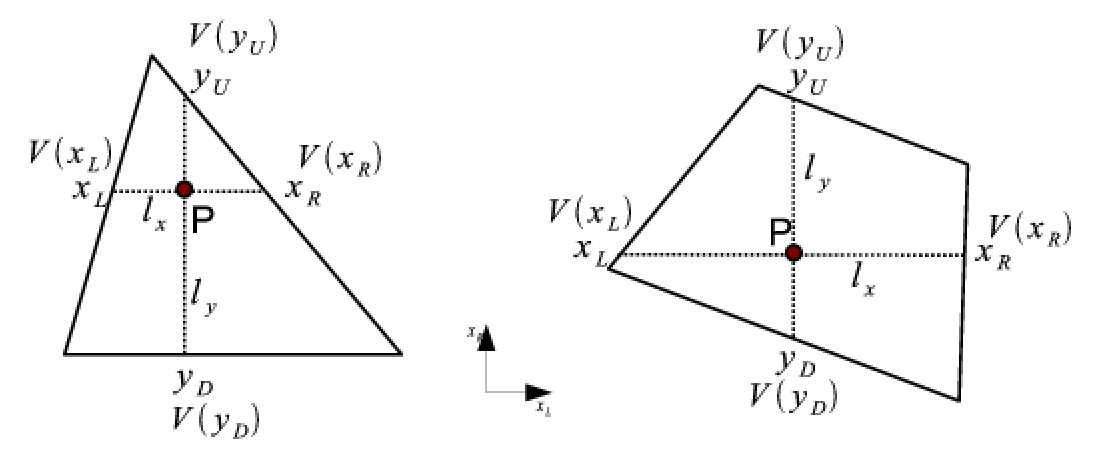
\includegraphics[scale=0.60]{RWPT/figures/DerivativeScheme.eps}
\caption{Spatial derivatives of velocity for a particle in triangular and quadrilateral elements: $x _L$ and $x _R$ are the intersectional points of the element edges with an extension of a  line parallel to the global $x$ axis at which velocities are $V(x _L)$ and $V(x _R)$, $y _D$ and $y _U$ are the intersectional points of the element edge from down to up with extension of the line parallel to the global $y$ axis at which velocities are $V(y _D)$ and $V(y _U)$, $z _S$ and $z _N$ are the intersectional points of the element edge from south to north with extension of the line parallel to the global $z$ axis at which velocities are $V(z _S)$ and $V(z _N)$, and $l _x$, $l _y$, and $l _z$ are the length of each intersectional line respectively}
\label{DerivativeVelocity}
\end{figure}


Thus, the derivatives of the dispersion coefficients are as follows \cite{hH02}

\begin{equation}\label{DerivativeDispersionCoefficient}
\begin{array}{lllllllll}
& \frac{\partial D _{xx}}{\partial x}=V _x\frac{\partial V _x}{\partial x}\left [
\alpha _L \left (\frac {2}{V} - \frac {V _x ^2}{V^3} \right ) - \alpha _T \frac {V _y ^2 + V _z ^2}{V^3} \right ] \\
& \frac{\partial D _{xy}}{\partial y}=(\alpha _L - \alpha _T)\left [\frac{\partial V _y}{\partial y}
\frac{V _x}{V} - \frac{V _x V _y^2}{V^3} \frac{\partial V _y}{\partial y} \right ] \\
& \frac{\partial D _{xz}}{\partial z}=(\alpha _L - \alpha _T)\left [\frac{\partial V _z}{\partial z}
\frac{V _x}{V} - \frac{V _x V _z^2}{V^3} \frac{\partial V _z}{\partial z} \right ] \\
& \frac{\partial D _{yy}}{\partial y}=V _y\frac{\partial V _y}{\partial y}\left [
\alpha _L \left (\frac {2}{V} - \frac {V _y ^2}{V^3} \right ) - \alpha _T \frac {V _x ^2 + V _z ^2}{V^3} \right ] \\
& \frac{\partial D _{yx}}{\partial x}=(\alpha _L - \alpha _T)\left [\frac{\partial V _x}{\partial x}
\frac{V _y}{V} - \frac{V _y V _x^2}{V^3} \frac{\partial V _x}{\partial x} \right ] \\
& \frac{\partial D _{yz}}{\partial z}=(\alpha _L - \alpha _T)\left [\frac{\partial V _z}{\partial z}
\frac{V _y}{V} - \frac{V _y V _z^2}{V^3} \frac{\partial V _z}{\partial z} \right ] \\
& \frac{\partial D _{zz}}{\partial z}=V _z\frac{\partial V _z}{\partial z}\left [
\alpha _L \left (\frac {2}{V} - \frac {V _z ^2}{V^3} \right ) - \alpha _T \frac {V _x ^2 + V _y ^2}{V^3} \right ] \\
& \frac{\partial D _{zx}}{\partial x}=(\alpha _L - \alpha _T)\left [\frac{\partial V _x}{\partial x}
\frac{V _z}{V} - \frac{V _z V _x^2}{V^3} \frac{\partial V _x}{\partial x} \right ] \\
& \frac{\partial D _{zy}}{\partial y}=(\alpha _L - \alpha _T)\left [\frac{\partial V _y}{\partial y}
\frac{V _z}{V} - \frac{V _z V _y^2}{V^3} \frac{\partial V _y}{\partial y} \right ] \\
\end{array}
\end{equation}

Because velocity is not derivable at the interface of two adjacent element in a nonuniform flow, computing dispersion coefficient derivatives by using a finite element approach would yield erroneous values \cite{hH02}. To prevent the errors, a particle is coded to have information of an element index and the velocity estimation is continuous even at the elemental boundaries in this method. Thus, the derivatives of dispersion coefficients will be computed accordingly. This is an improved approach from the work by \cite{hH02}.


\section{Transport: Advection and Dispersion}

\subsubsection*{Purpose}
%
To verify advective dispersive transport, a two-dimensional homogeneous aquifer is chosen to test the proposed RWPT method and the simulated particle distribution is converted to concentration contours.

\subsubsection*{Model description}
%
The dimension of the model domain is 100 $m$ by 60 $m$ where the uniform velocity field is held constant at 0.5 $md^{-1}$ in the $x$ direction. The hydraulic conductivity is set as $10^{-5}$ $md^{-1}$ and the head gradient of one in the $x$ direction is set by assigning two constant boundary conditions along both left and right sides. The longitudinal and transverse dispersivities are chosen to be isotropic with a length of 0.1 $m$. This converts to isotropic dispersion coefficients of 0.05 $m^2d^{-1}$. The initial source load is applied to an area with dimensions of 0.1 $m$ by 0.1 $m$ to have an initial concentration of $C _0=1$ $kg m^{-3}$.
Figure \ref{ModelSchematic} provides a schematic description of the test problem for the two-dimensional homogeneous aquifer. The domain is discretized with quadrilateral elements of 0.5 $m$ by 0.5 $m$. The same grid density is also used for converting particle distributions to element concentrations.

The stated problem can be solved with an analytical solution provided by \cite{aO61}.
\begin{equation}\label{ogata}
C\left( {x,y,t} \right) = \frac{{C_0 A}}{{4\pi t\sqrt {D_{xx} + D_{yy} } }}\exp\left[ { - \frac{{\left( {x - x_0 } \right)^2 }}{{4D_{xx} t}} - \frac{{\left( {y - y_0 } \right)^2 }}{{4D_{yy} t}}} \right]
\end{equation}
This allows to evaluate the computational accuracy of the proposed method.

\begin{figure}[h]
\centering
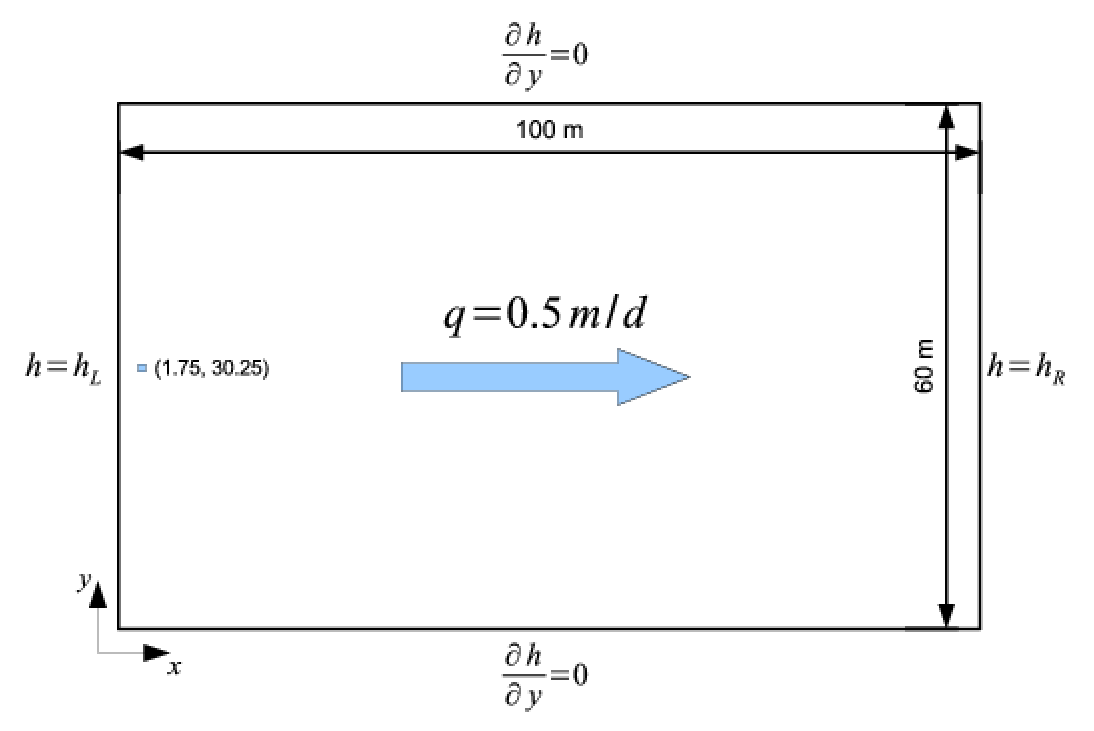
\includegraphics[scale=0.45]{RWPT/figures/ModelSchematic.eps}
\caption{Schematic description of the two-dimensional aquifer and the boundary conditions of the flow system}
\label{ModelSchematic}
\end{figure}

\subsubsection*{Results}
%
The comparison with the analytical solution is provided in Figure \ref{TransportHomo50K}. As can be seen, the result of the RWPT method shows good agreement with the analytical solution. The number of particles used for this simulation is 50000. This is significantly less than the number of particles reported by \cite{aH03}, who reported that up to 2.5 million particles were necessary to achieve smoothness of the solution due to oscillations around the contours. As the oscillations observed here for the method proposed are smaller than reported by \cite{aH03}, the proposed method allows to dramatically reduce the number of particles required for a smooth solution by about two orders of magnitude. This shows that the proposed method is both accurate and efficient.
In addition, the several numbers of particles used to solve the same problem produces particle clouds as in Fig. \ref{ParticleClouds}. However, the problem for only 1000 particles is used for the purpose of the benchmark test to reduce computation time.
%-------------------------------------------------
\begin{figure}[h]
\centering
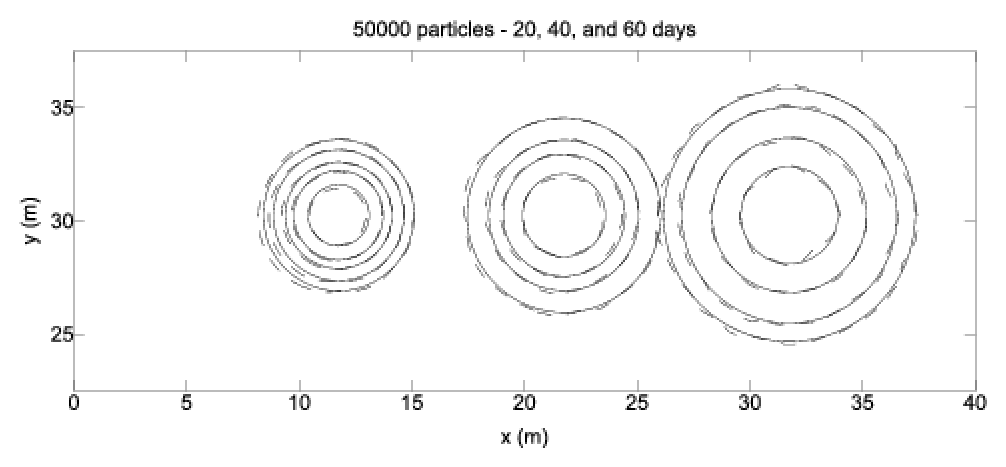
\includegraphics[scale=0.60]{RWPT/figures/TransportHomo50K.eps}
\caption{Transport results of the RWPT method compared with the
analytical solution \cite{aO61} for 50000 particles at 20, 40,
and 60 days: The solid line is the analytical solution, the dotted
line is the RWPT result. Contour lines are shown for $C=2.6e^{-4}$, $1.6e^{-4}$, $1.0e^{-4}$, and $4e^{-5}$.} 
\label{TransportHomo50K}
\end{figure}

\begin{figure}[h]
\centering
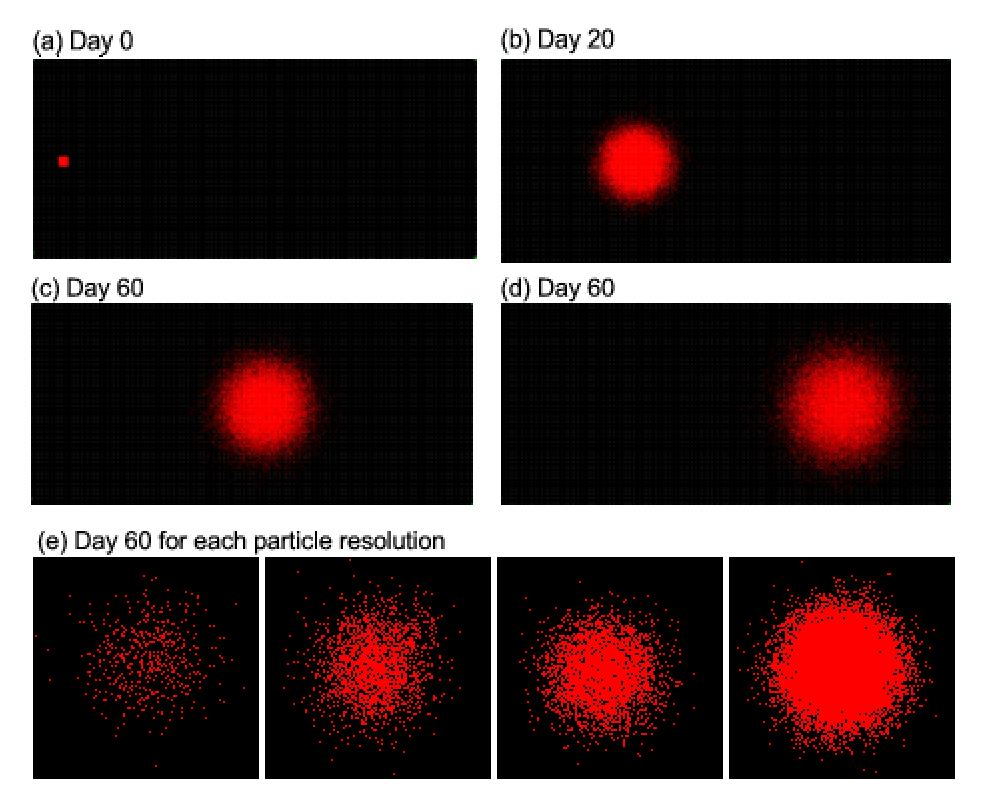
\includegraphics[scale=0.60]{RWPT/figures/ParticleClouds.eps}
\caption{(a-d)Particle clouds of 50000 particles at 0, 20, 40, and 60 days, (e) Particle clouds of 1000, 5000, 10000, and 50000 at 60 days}
\label{ParticleClouds}
\end{figure}

\begin{tabular}{|l|l|l|}
\hline
Benchmark & Problem type	& Path in benchmark deposit \\
\hline	
quad\_homo	& RWPT	& benchmarks $\backslash$RWPT$\backslash$Veri1000 \\
\hline	
\end{tabular}

%-------------------------------------------------


\section{Transport: Sorption-desorption and Filtration}

\subsubsection*{Problem definition}
%
Harter et al.\textquoteright s experiment \cite{HarWag:2000} used a 10 cm long acrylic column filled with sand and fully saturated with water. A constant, uninterrupted flow rate was established with a peristaltic pump. The following sequence of solutions was injected during the experiment: 10 pore volumes DTW (degassed tap water), 2.5 pore volumes NaCl - tap water solution, 10 pore volumes DTW, 2.5 pore volumes \emph{Cryptosporidium parvum} solutions ($1\times10^5$ oocysts per mL), 250 pore volumes DTW. The outflow was continuously collected for determination of concentration.

NaCl - tap water solution is used as tracer. The \emph{Cryptosporidium parvum} can be classified as biological colloid. Colloids moving in porous media experience advection, dispersion, sorption-desorption, and filtration. A one-dimensional homogeneous aquifer is chosen to verify colloids transport in the experiment. Figure \ref{ExperimentSchematic} shows the schematic discription of the experiment.

\begin{figure}[h]
\centering
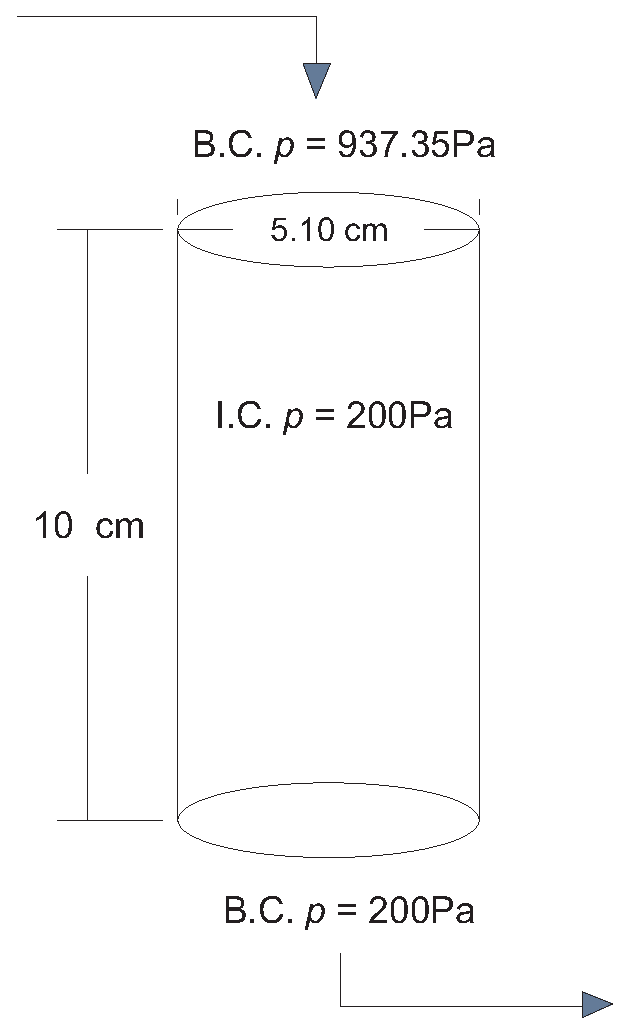
\includegraphics[scale=0.35]{RWPT/figures/ExperimentSchematic.eps}
\caption{Schematic description of the Harter experiment}
\label{ExperimentSchematic}
\end{figure}

\subsubsection*{Governing equations and analytical solution}
%
For the one-dimensional transport including sorption/desorption and filtration through a homogeneous medium the following differential equation \ref{colloid transeq} is applied.
\begin{equation}\label{colloid transeq}
\frac{\partial C}{\partial t} + \frac{\rho_b}{\theta} \frac{\partial S}{\partial t} = v \alpha_L \frac{\partial^2 C}{\partial x^2} - v (\frac{\partial C}{\partial x} + \lambda C)
\end{equation}
{\small
with
\begin{itemize}
\item[$C$] -- dissolved concentration (kg$\cdot$m$^{-3}$),
\item[$S$] -- sorbed concentration(kg$\cdot$kg$^{-1}$),
\item[$t$] -- time (s),
\item[$\rho_b$] -- bulk density (kg$\cdot$m$^{-3}$),
\item[$\theta$] -- porosity (-),
\item[$v$] -- velocity (m$\cdot$s$^{-1}$),
\item[$\alpha_L$] -- longitudinal dispertivity (m),
\item[$x$] -- distance (m),
\item[$\lambda$] -- filtration coefficient (m$^{-1}$).
\end{itemize}
}

The instantaneous, linear sorption model assumes that
\begin{equation}\label{colloid sorption model}
S = K_{d} C
\end{equation}
where $K_{d}$ is the partitioning coefficient ($m^3 \cdot kg^{-1}$). The retardation coefficient $R$ is
\begin{equation}\label{colloid retardation coefficient}
R = 1 + \frac{\rho_b}{\theta} K_{d}
\end{equation}
The dispersion coefficient in $x$-direction $D_{xx}$ ($m^2 \cdot s^{-1}$) is
\begin{equation}\label{colloid dispersion x}
D_{xx} = v \alpha_L
\end{equation}
The analytical solution for a pulse input (inject time from 0 to $\tau$) is:
\begin{eqnarray}\label{colloid analytical 1}
C = & \frac{1}{2} C_0 &
\mbox{\hspace{-1.5ex}}\mbox{\hspace{-1.5ex}}
\left[
\exp
\left(
\frac{v x(1-\gamma)}{2 D_{xx}}
\right)
\mathrm{erfc}
\left(
\frac{x-v\gamma t/R}{2 \sqrt{D_{xx} t/R}}
\right)
\right. \nonumber\\[0.5ex]
& &
+\left.
\exp
\left(
\frac{v x(1+\gamma)}{2 D_{xx}}
\right)
\mathrm{erfc}
\left(
\frac{x+v\gamma t/R}{2 \sqrt{D_{xx} t/R}}
\right)
\right]
\end{eqnarray}
for $t \in (0, \tau) $ ,

\begin{eqnarray}\label{colloid analytical 2}
C = & \frac{1}{2} C_0 &
\mbox{\hspace{-1.5ex}} \mbox{\hspace{-1.5ex}}
\left[
\exp
\left(
\frac{v x(1-\gamma)}{2 D_{xx}}
\right)
\mathrm{erfc}
\left(
\frac{x-v \gamma t/R}{2 \sqrt{D_{xx} t/R}}
\right)
\right. \nonumber\\[0.5ex]
& &
+\left.
\exp
\left(
\frac{v x(1+\gamma)}{2 D_{xx}}
\right)
\mathrm{erfc}
\left(
\frac{x + v \gamma t/R}{2 \sqrt{D_{xx} t/R}}
\right)
\right. \nonumber\\[0.5ex]
& &
-\left.
\exp
\left(
\frac{v x(1-\gamma)}{2 D_{xx}}
\right)
\mathrm{erfc}
\left(
\frac{x - v\gamma (t - \tau)/R}{2 \sqrt{D_{xx} (t - \tau)/R}}
\right)
\right. \nonumber\\[0.5ex]
& &
-\left.
\exp
\left(
\frac{v x(1+\gamma)}{2 D_{xx}}
\right)
\mathrm{erfc}
\left(
\frac{x + v \gamma (t - \tau)/R}{2 \sqrt{D_{xx} (t - \tau)/R}}
\right)
\right]
\end{eqnarray}
for $t \in (\tau, \infty) $ , where

\begin{equation}\label{colloid analytical 3}
\gamma = \sqrt{1 + 4  v  \lambda  R  D_{xx} / v^2}
\end{equation}

\subsubsection*{Model description}
%
The calculation area of the column is simplified to a line with the length of 0.1m. For the numerical model 100 elements and 101 nodes are included. Head gradient is set by giving two constant pressures at both left and right boundaries to establish a uniform velocity field. Particles are loaded near the left boundary for several time steps. The longitudinal dispersivity is chosen to be isotropic with a length of 0.005$m$. The sorption-desorption process is described by the two-rate model from Johnson et al.\cite{JohBluLog:95}. Filtration is described by using the filtration coefficient. 

The two-rate model provides for a large number of particles to be released initially, followed by a slow release of attached particles. It is given by
\begin{equation}\label{colloid two-rate}
N/N_{0} = A e^{-k_{1}t} + (1-A) e^{-k_{2}t}
\end{equation}
where $N$ is the number of particles remaining on the medium at time $t$, $N_{0}$ is the initial number of particles on the medium at the time of initial sorption, $A$ is a weighting factor, $k_{1}$ and $k_{2}$ are the fast and slow sorption rate coefficient, respectively. Relative parameters are listed in Tab.~\ref{colloid transport parameters}.

\begin{table}[ht]
\begin{center}
\begin{tabular}{llll}
\toprule
Parameter 						& Value \\
\midrule
\multicolumn{2}{c}{\textit{Advection-dispersion parameters}} \\
permeability $k$				& $\unit[1.114476^{-11}]{m^2}$  \\
longitudinal dispersivity $\alpha_L$ 				& $\unit[0.005]{m}$  \\
porosity(colloid) $\theta$ 			& 0.42  \\
porosity(tracer) $\theta$ 			& 0.5  \\
\cmidrule{1-4}
\multicolumn{2}{c}{\textit{Sorption-desorption parameters}}\\
$A$            			& 0.9  \\ 
$k_{1}$ 		    		& 0.1 \\
$k_{2}$ 		    		& 0.001 \\
\cmidrule{1-4}
\multicolumn{2}{c}{\textit{Filtration parameter}}\\
filtration coefficient $\lambda$ 			& $\unit[5.2]{m^{-1}}$  \\
\bottomrule
\end{tabular}
\end{center}
\caption{\label{colloid transport parameters}Model parameters for the column experiment.}
\end{table}

\subsubsection*{Results}
%
The number of pore volume($x$-axis) is calculated by
\begin{equation}\label{colloid pv}
P_{V} = \frac{v t}{L}
\end{equation}

The time step size is set by assigning $P_{V}$ to 0.01. The chloride in the column experiences only advection and dispersion, which means in the Equation \ref{colloid transeq}, $S = 0$, $\lambda = 0$. The comparison with the measurements from the experiment by Harter, the analytical solution, and the OGS simulation with mass transport method are shown in Figure \ref{Tracertransport}.

\begin{figure}[h]
\centering
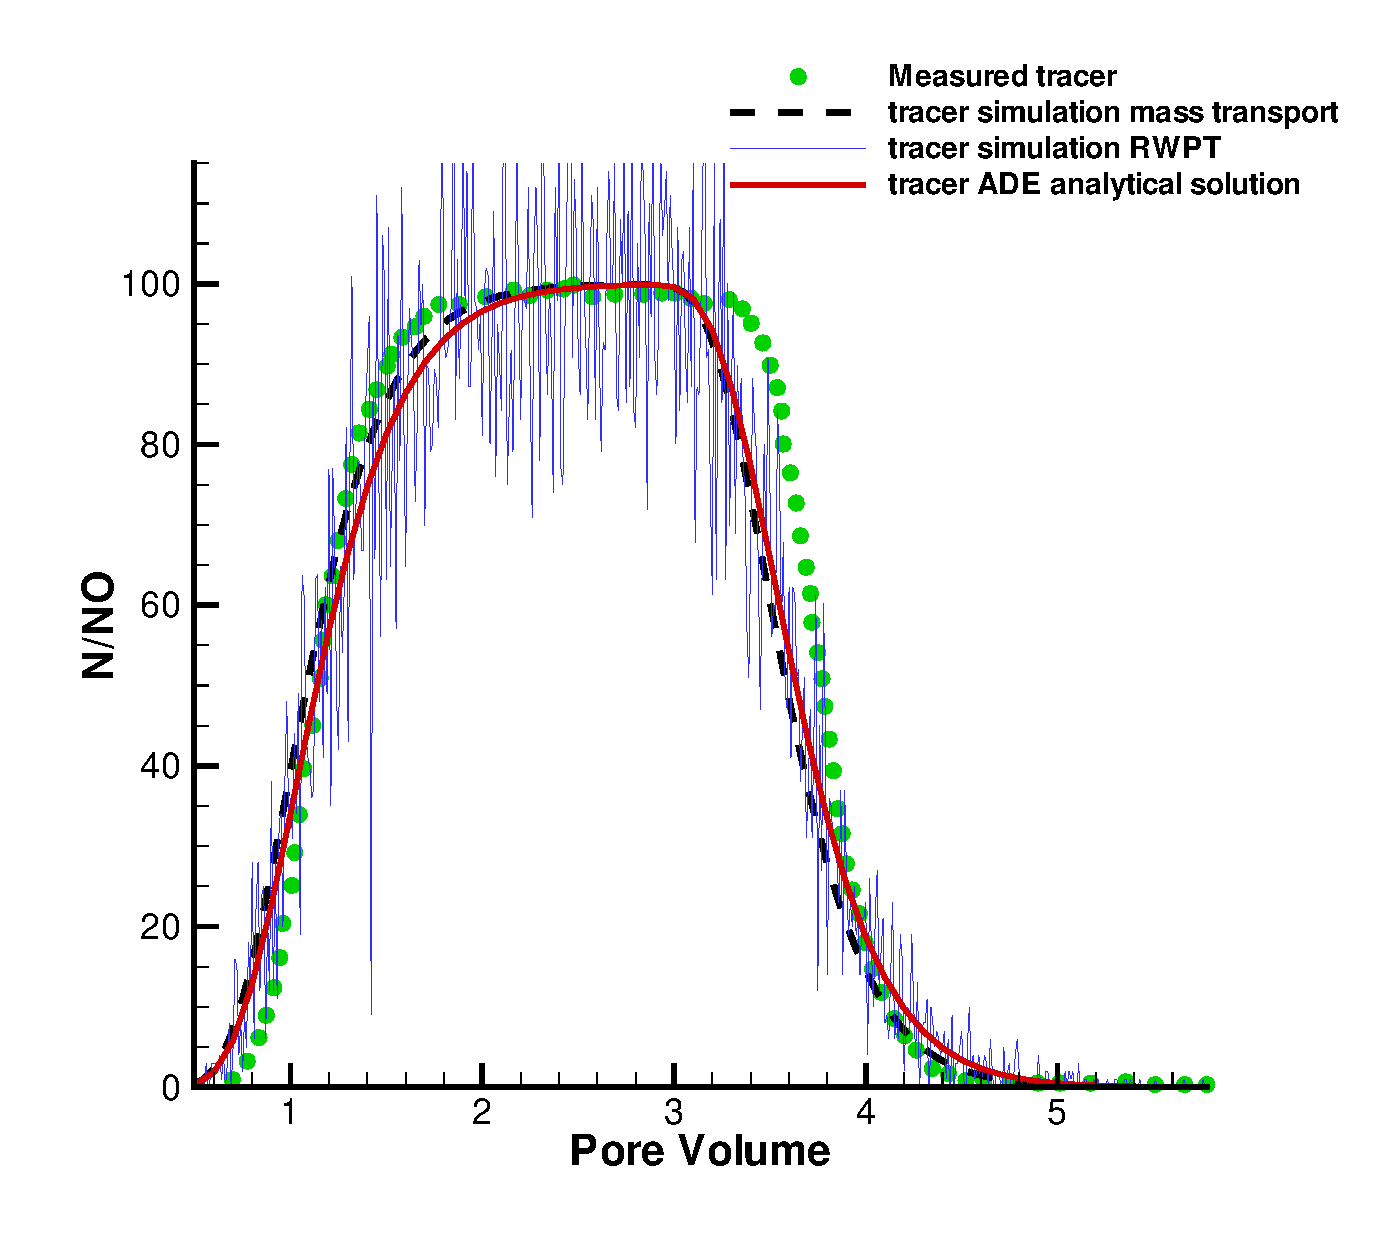
\includegraphics[scale=0.40]{RWPT/figures/Tracertransport.eps}
\caption{Tracer transport with advection and dispertion}
\label{Tracertransport}
\end{figure}

100 particles per time steps are injected for 250 time steps. The leaving particles from the right boundary are counted to obtain the corresponding breakthrough curves. The comparison with the measurements from the experiment by Harter are shown in Figure \ref{ColloidTransport}.

\begin{figure}[h]
\centering
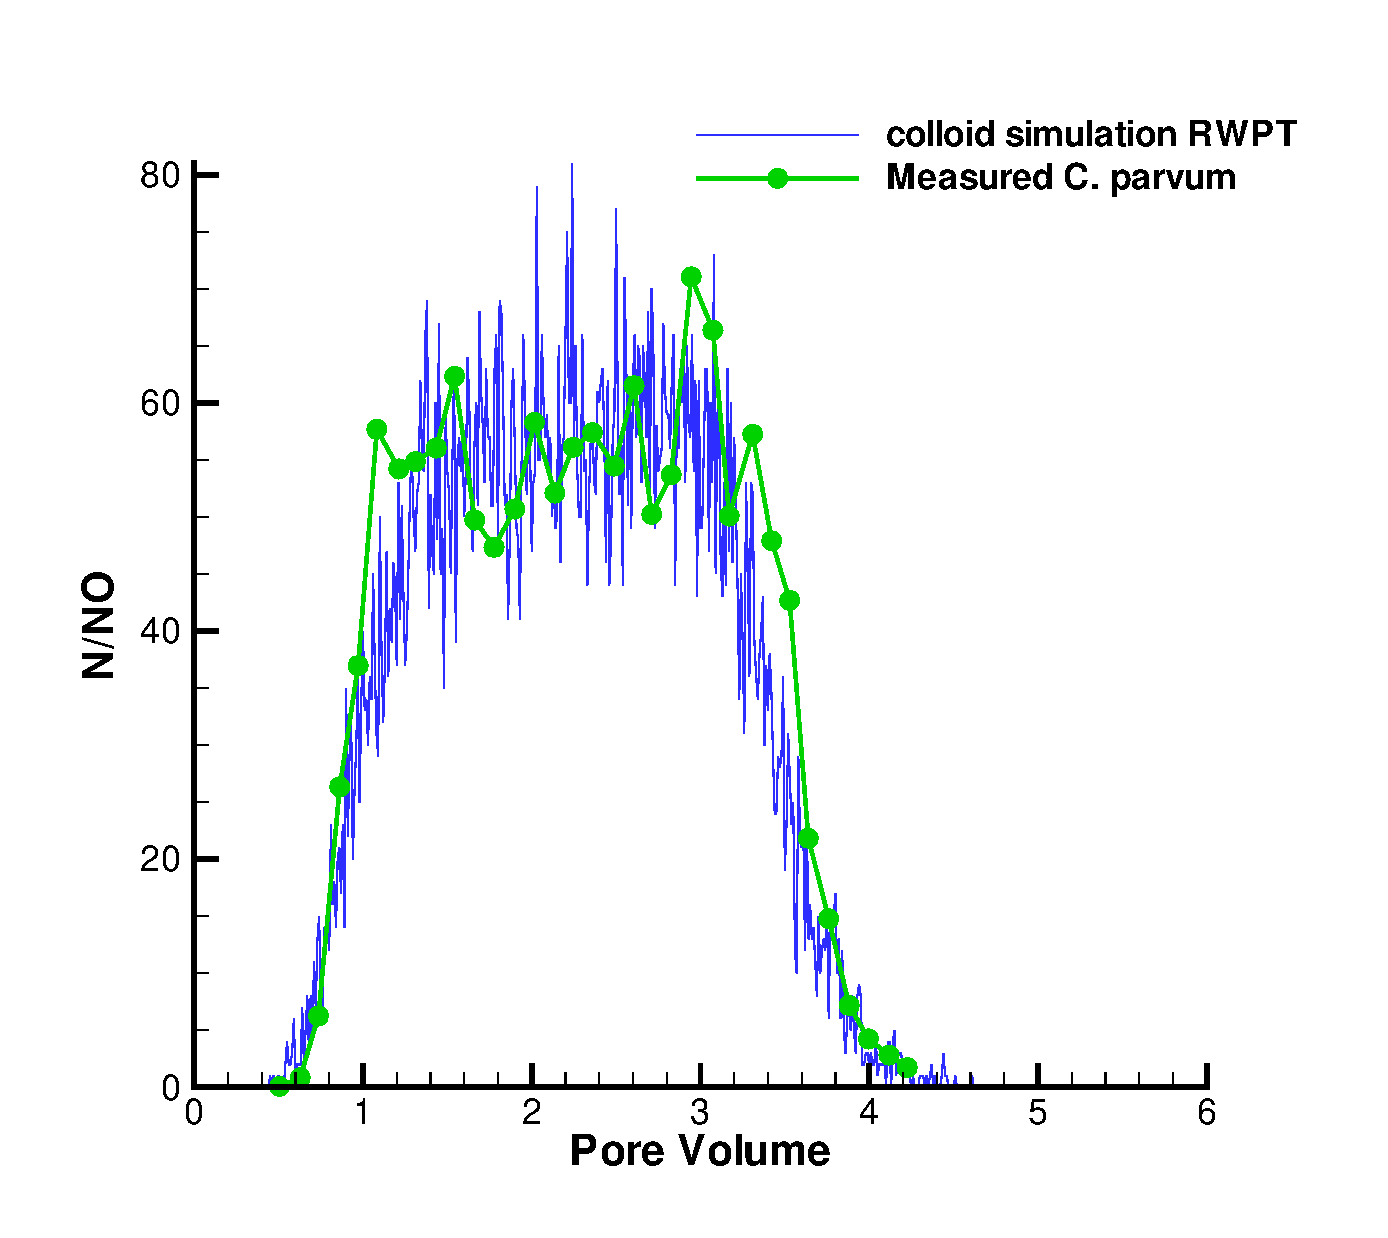
\includegraphics[scale=0.40]{RWPT/figures/ColloidTransport.eps}
\caption{Colloid transport with advection, dispersion, sorption-desorption and decay}
\label{ColloidTransport}
\end{figure}

\begin{tabular}{|l|l|l|}
\hline
Benchmark & Problem type	& Path in benchmark deposit \\
\hline	
colloid\_t	& RWPT	& benchmarks $\backslash$RWPT$\backslash$Harter \\
\hline	
\end{tabular}
